\section{Exercise 3: Random asymmetry}

\begin{itshape}
\small
To investigate the robustness of pattern retrieval against asymmetry in the weight matrix, consider now networks where for each pairs of nodes $\l(i, j\r)$, the directed connection from node $i$ to node $j$ is cut with probability $p_{cut}$. This will introduce asymmetry in the Hebbian weight matrix Eq. 1.

Set $c=0.1$ and $N = 200$. As in Ex. 2 calculate and plot the mean $\alpha_{N,max}$ for varying $p_{cut}$ with error bars (at least 10 repetitions). At which $p_{cut}$ does the maximal load drop below $50\%$ of the value estimated in Ex. 2? State the confidence interval.

Note: Bare in mind that the convergence assertion of Question 1.1 does not necessarily hold for $p_{cut} > 0$.
\end{itshape}

\paragraph*{}



\begin{figure}[H]
  \vspace{-20pt}
  \begin{center}
    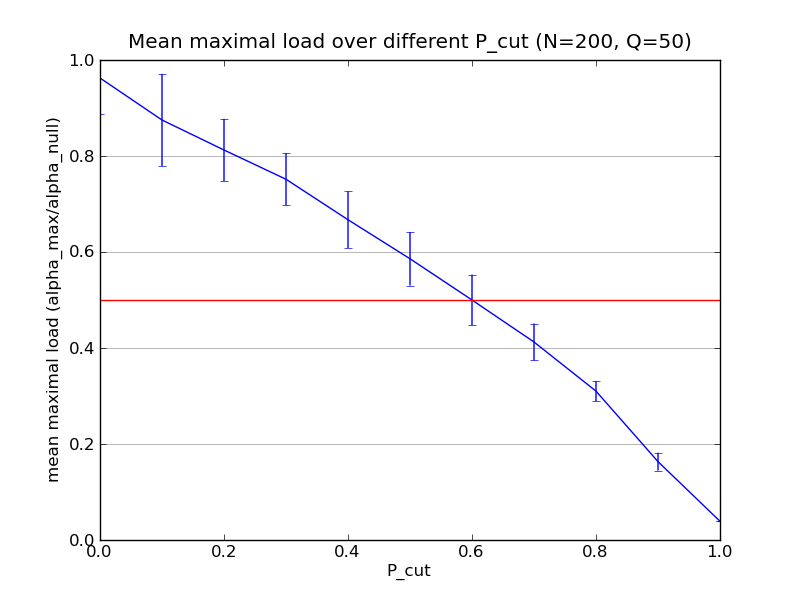
\includegraphics[width=0.6\textwidth]{dat/ex3-mean_max_load-N200-Q50-C95}
  \end{center}
  \vspace{-20pt}
  \caption{Exercise 3: Maximal load $\alpha_{N,max}$ averaged over 10 repetitions for varying $p_{cut}$ }
  \label{fig:exercise3}
  \vspace{-10pt}
\end{figure}

Figure \ref{fig:exercise3} shows the the $\alpha_{N,max}$ over varying $p_{cut}$. Table 

\begin{table}[H] 
\centering 
\begin{tabular}{|l|l|l|l|l|l|l|l|} 
\hline 
\begin{table}[H] 
\centering 
\begin{tabular}{|l|l|l|l|l|l|l|l|} 
\hline 
$P_{cut} & N & tests & C-level & maximal load & lower bound & upper bound & $P_{N,max}$\\ 
 \hline \hline 
0.0 & 200 & 10 & 95.0 $\%$  & 0.12 & 0.12 & 0.13 & 24.90 \\ 
0.1 & 200 & 10 & 95.0 $\%$  & 0.11 & 0.11 & 0.11 & 22.70 \\ 
0.2 & 200 & 10 & 95.0 $\%$  & 0.11 & 0.10 & 0.11 & 21.10 \\ 
0.3 & 200 & 10 & 95.0 $\%$  & 0.10 & 0.10 & 0.10 & 19.20 \\ 
0.4 & 200 & 10 & 95.0 $\%$  & 0.09 & 0.09 & 0.09 & 17.50 \\ 
0.5 & 200 & 10 & 95.0 $\%$  & 0.08 & 0.08 & 0.08 & 15.40 \\ 
0.6 & 200 & 10 & 95.0 $\%$  & 0.07 & 0.06 & 0.07 & 13.10 \\ 
0.7 & 200 & 10 & 95.0 $\%$  & 0.05 & 0.05 & 0.05 & 9.90 \\ 
0.8 & 200 & 10 & 95.0 $\%$  & 0.04 & 0.04 & 0.04 & 7.80 \\ 
0.9 & 200 & 10 & 95.0 $\%$  & 0.02 & 0.02 & 0.02 & 4.30 \\ 
1.0 & 200 & 10 & 95.0 $\%$  & 0.01 & 0.01 & 0.01 & 1.00 \\ 
	
\hline
\end{tabular}
\label{tbl:exercise3_CI}
\caption{Table giving the confidence intervals for all data points in figure \ref{fig:exercise3}.}
\end{table} 

With increasing $p_{cut}$ the maximal load decreases. At $p_{cut} = 0.6$ the maximal load drops below $50\%$ of the value estimated in exercise 2. The confidence intervals are listed in table \ref{tbl:exercise3_CI}
